\subsection{Проектирование и разработка серверной части программного средства}
\label{sec:design:server}

\subsubsection{} Этапы разработки программного средства
\label{sec:design:server:overview}

Архитектурный стиль разделения функциональности программной системы на уровни поднимает сразу несколько проблем. Их решение в типичном случае заключается в выполнении следующих этапов~\cite{application_architecture_guide}:

\begin{enumerate}
	\item определение стратегии разбиения на уровни;
	\item определение уровней;
	\item распределение функциональности по уровням и компонентам;
	\item уточнение количества уровней: при необходимости некоторые из них объединяются;
	\item установление правил взаимодействия уровней;
	\item идентификация функциональности, которая используется на всех\linebreak уровнях (cross cutting concerns);
	\item определение интерфейсов уровней;
	\item выбор стратегии развертывания;
	\item выбор конкретных протоколов взаимодействия.
\end{enumerate}

К данному этапу разработки дипломного проекта выполнены шаги с \ref{sec:design:server:overview}а по \ref{sec:design:server:overview}д. Шаг \ref{sec:design:server:overview}е вследствие использования различных программных средств, применяемых на уровнях, будет выполняться позднее -- на соответствующих уровнях.

Таким образом, следующий этап -- это определение интерфейсов уровней. СУБД имеет заранее определенный интерфейс, установленный ее разработчиком. Предполагается, что из остальных двух частей программной системы инициатором любых действий будет являться клиентская. Следовательно, единственный межуровневый интерфейс, который следует определить -- это интерфейс серверной части.

Веб-приложения, в стиле которых планируется создание клиентской части, обычно запускаются большим числом пользователей. Таким образом очевидна автономность и независимость частей проектируемой программной системы. Исходя из этих соображений, целесообразным является применение сервис-ориентированного архитектурного стиля.

\subsubsection{} Программный интерфейс серверной части
\label{sec:design:server:interface}

Предварительным условием для проектирования серверной части приложения является определение его интерфейса в высокоуровневых терминах предметной области. Таким образом, далее приведены методы его API, которые основаны на функциональных требованиях, определенных в подразделе~\ref{sec:domain:specification}:

\begin{itemize}
	\item метод регистрации пользователя системы, принимающий адрес электронной почты, хеш-сумму пароля, строку соли и название применявшегося алгоритма хеширования;
	\item метод смены пароля, также принимающий хеш-сумму пароля, соль и название алгоритма;
	\item метод смены пользователем электронной почты;
	\item метод аутентификации, принимающий хеш пароля и адрес электронной почты;
	\item метод восстановления пароля, принимающий адрес электронной почты;
	\item метод извлечения персональных данных пользователей;
	\item метод изменения фамилии, имени, отчества пользователя;
	\item метод изменения значения поля <<О себе>> пользователя;
	\item метод смены роли пользователя, принимающий объект сущности пользователя и роль, которую желается установить;
	\item метод подачи заявки на роль студента, принимающий номер группы;
	\item метод подачи заявки на роль преподавателя, в качестве параметра в котором выступает объект кафедры, сотрудником которой является преподаватель;
	\item методы подтверждения и отклонения заявок студентов;
	\item методы подтверждения и отклонения заявок преподавателей;
	\item метод, принимающий диапазон дат и номер группы и возвращающий список занятий;
	\item метод, который аналогичен предыдущему, но принимающий вдобавок номер подгруппы;
	\item метод, принимающий диапазон дат и фамилию, имя и отчество преподавателя и возвращающий список его занятий;
	\item метод, возвращающий список изучаемых студентов дисциплин;
	\item метод, возвращающий список дисциплин преподавателя;
	\item метод создания индивидуального задания преподавателем, принимающий номера групп и файл с условием задания;
	\item методы модификации условия индивидуального задания, включающие поиск и собственно изменение;
	\item метод отправки результатов выполнения заданий студентом;
	\item метод отклонения результатов задания преподавателем;
	\item метод оценивания результатов;
	\item метод извлечения всех результатов выполнения заданий, полученных и не проверенных преподавателем;
	\item метод добавления преподавателем файла учебно-методических материалов;
	\item метод получения прогресса выполнения заданий по всем предметам студента, в том числе полученные оценки (при их наличии);
	\item метод отправки сообщения одного пользователя другому;
	\item метод отправки сообщения с прикреплением;
	\item метод получения списка сообщения, переданных между двумя пользователями, принимающий помимо идентификационных номеров пользователей число сообщения для возврата и смещение, с какого сообщения начинать их выборку;
	\item метод создания объявления пользователя;
	\item метод извлечения объявлений пользователя, также принимающий их число и номер, с которого начинать выборку;
	\item метод получения списка студентов;
	\item метод получения списка студентов с их оценками по индивидуальным заданиям, а также с отметками посещения;
	\item метод совершения проверки посещения группой занятия;
	\item метод поиска пользователей;
	\item метод поиска преподавателей;
	\item метод поиска факультетов;
	\item метод поиска кафедр;
	\item метод поиска групп студентов;
	\item метод, возвращающий все группы факультета;
	\item методы выборки, создания и модификации специальностей\linebreakфакультета;
	\item методы выборки, создания и модификации программ специальностей.
\end{itemize}

На рисунке~\ref{fig:design:server:interface:server_algorithm} приведена схема алгоритма обработки запросов перечисленных методов программного интерфейса серверной частью приложения. Далее приведены архитектурные решения, которые были применены при реализации данной части программной системы. 

\begin{sidewaysfigure}
\centering
	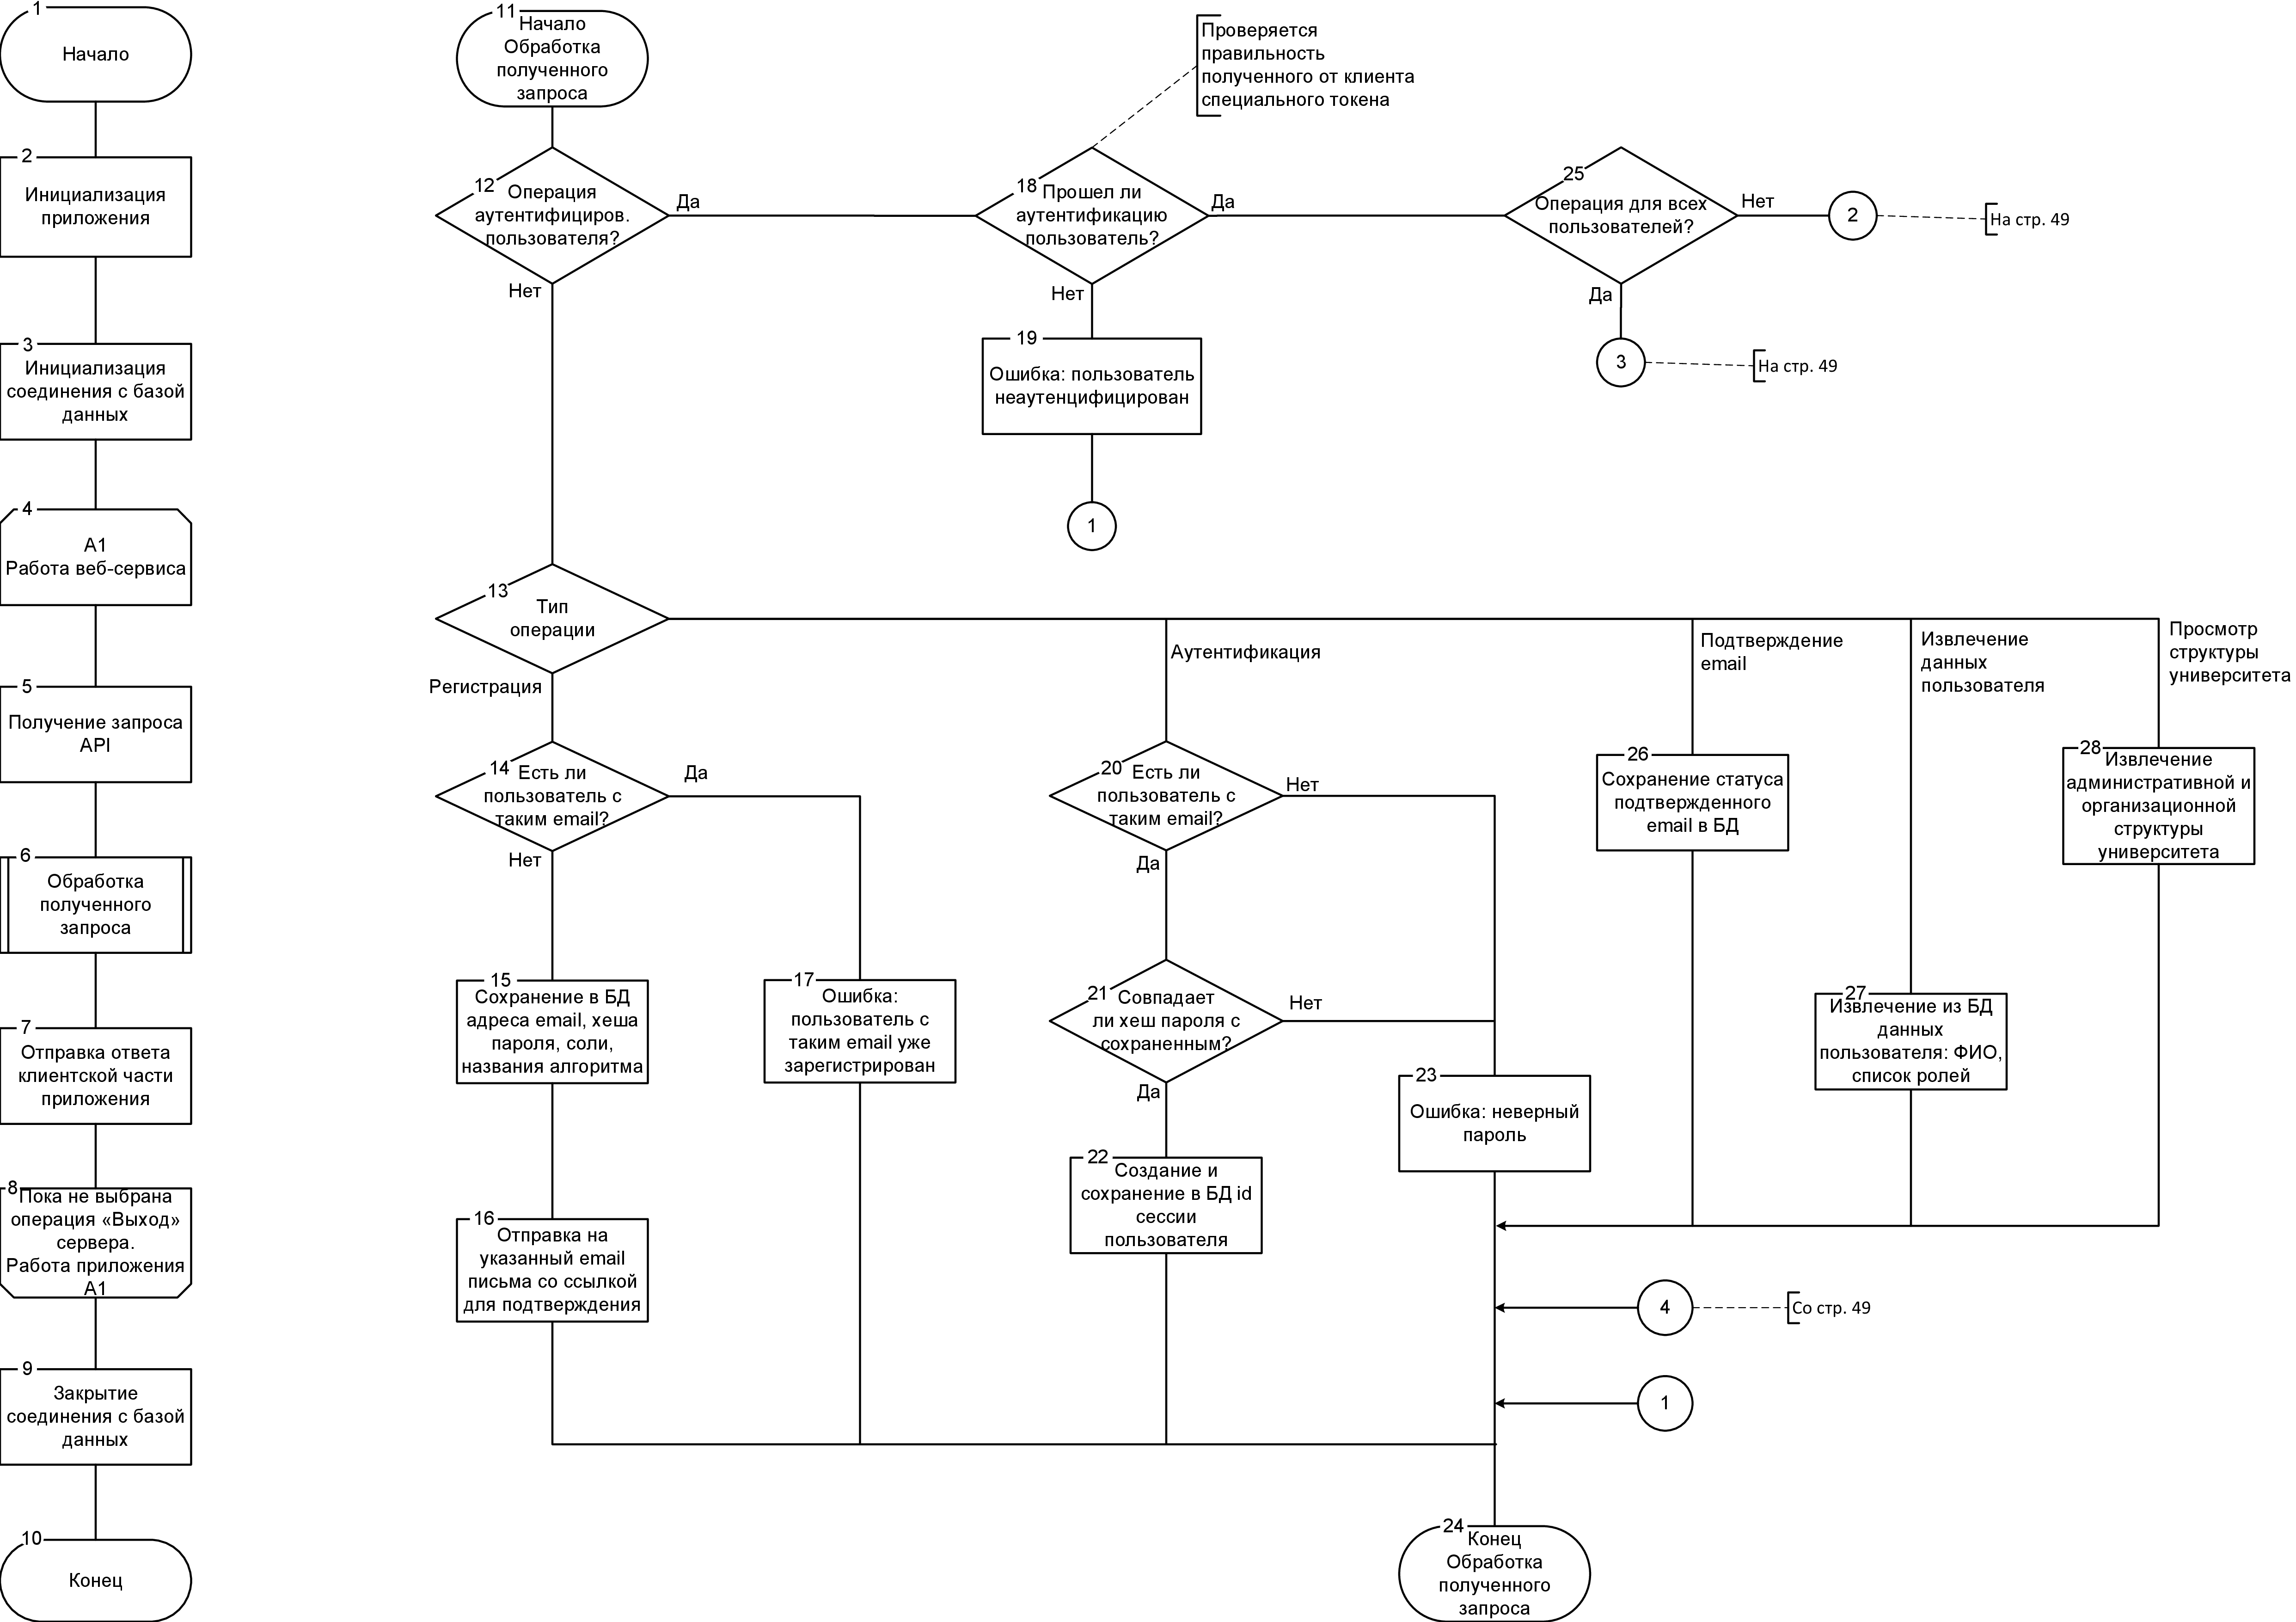
\includegraphics[scale=0.275]{server_algorithm_1.png}
	\caption{Схема программы серверной части программного средства}
	\label{fig:design:server:interface:server_algorithm}
\end{sidewaysfigure}

\begin{sidewaysfigure}
\ContinuedFloat
\centering
	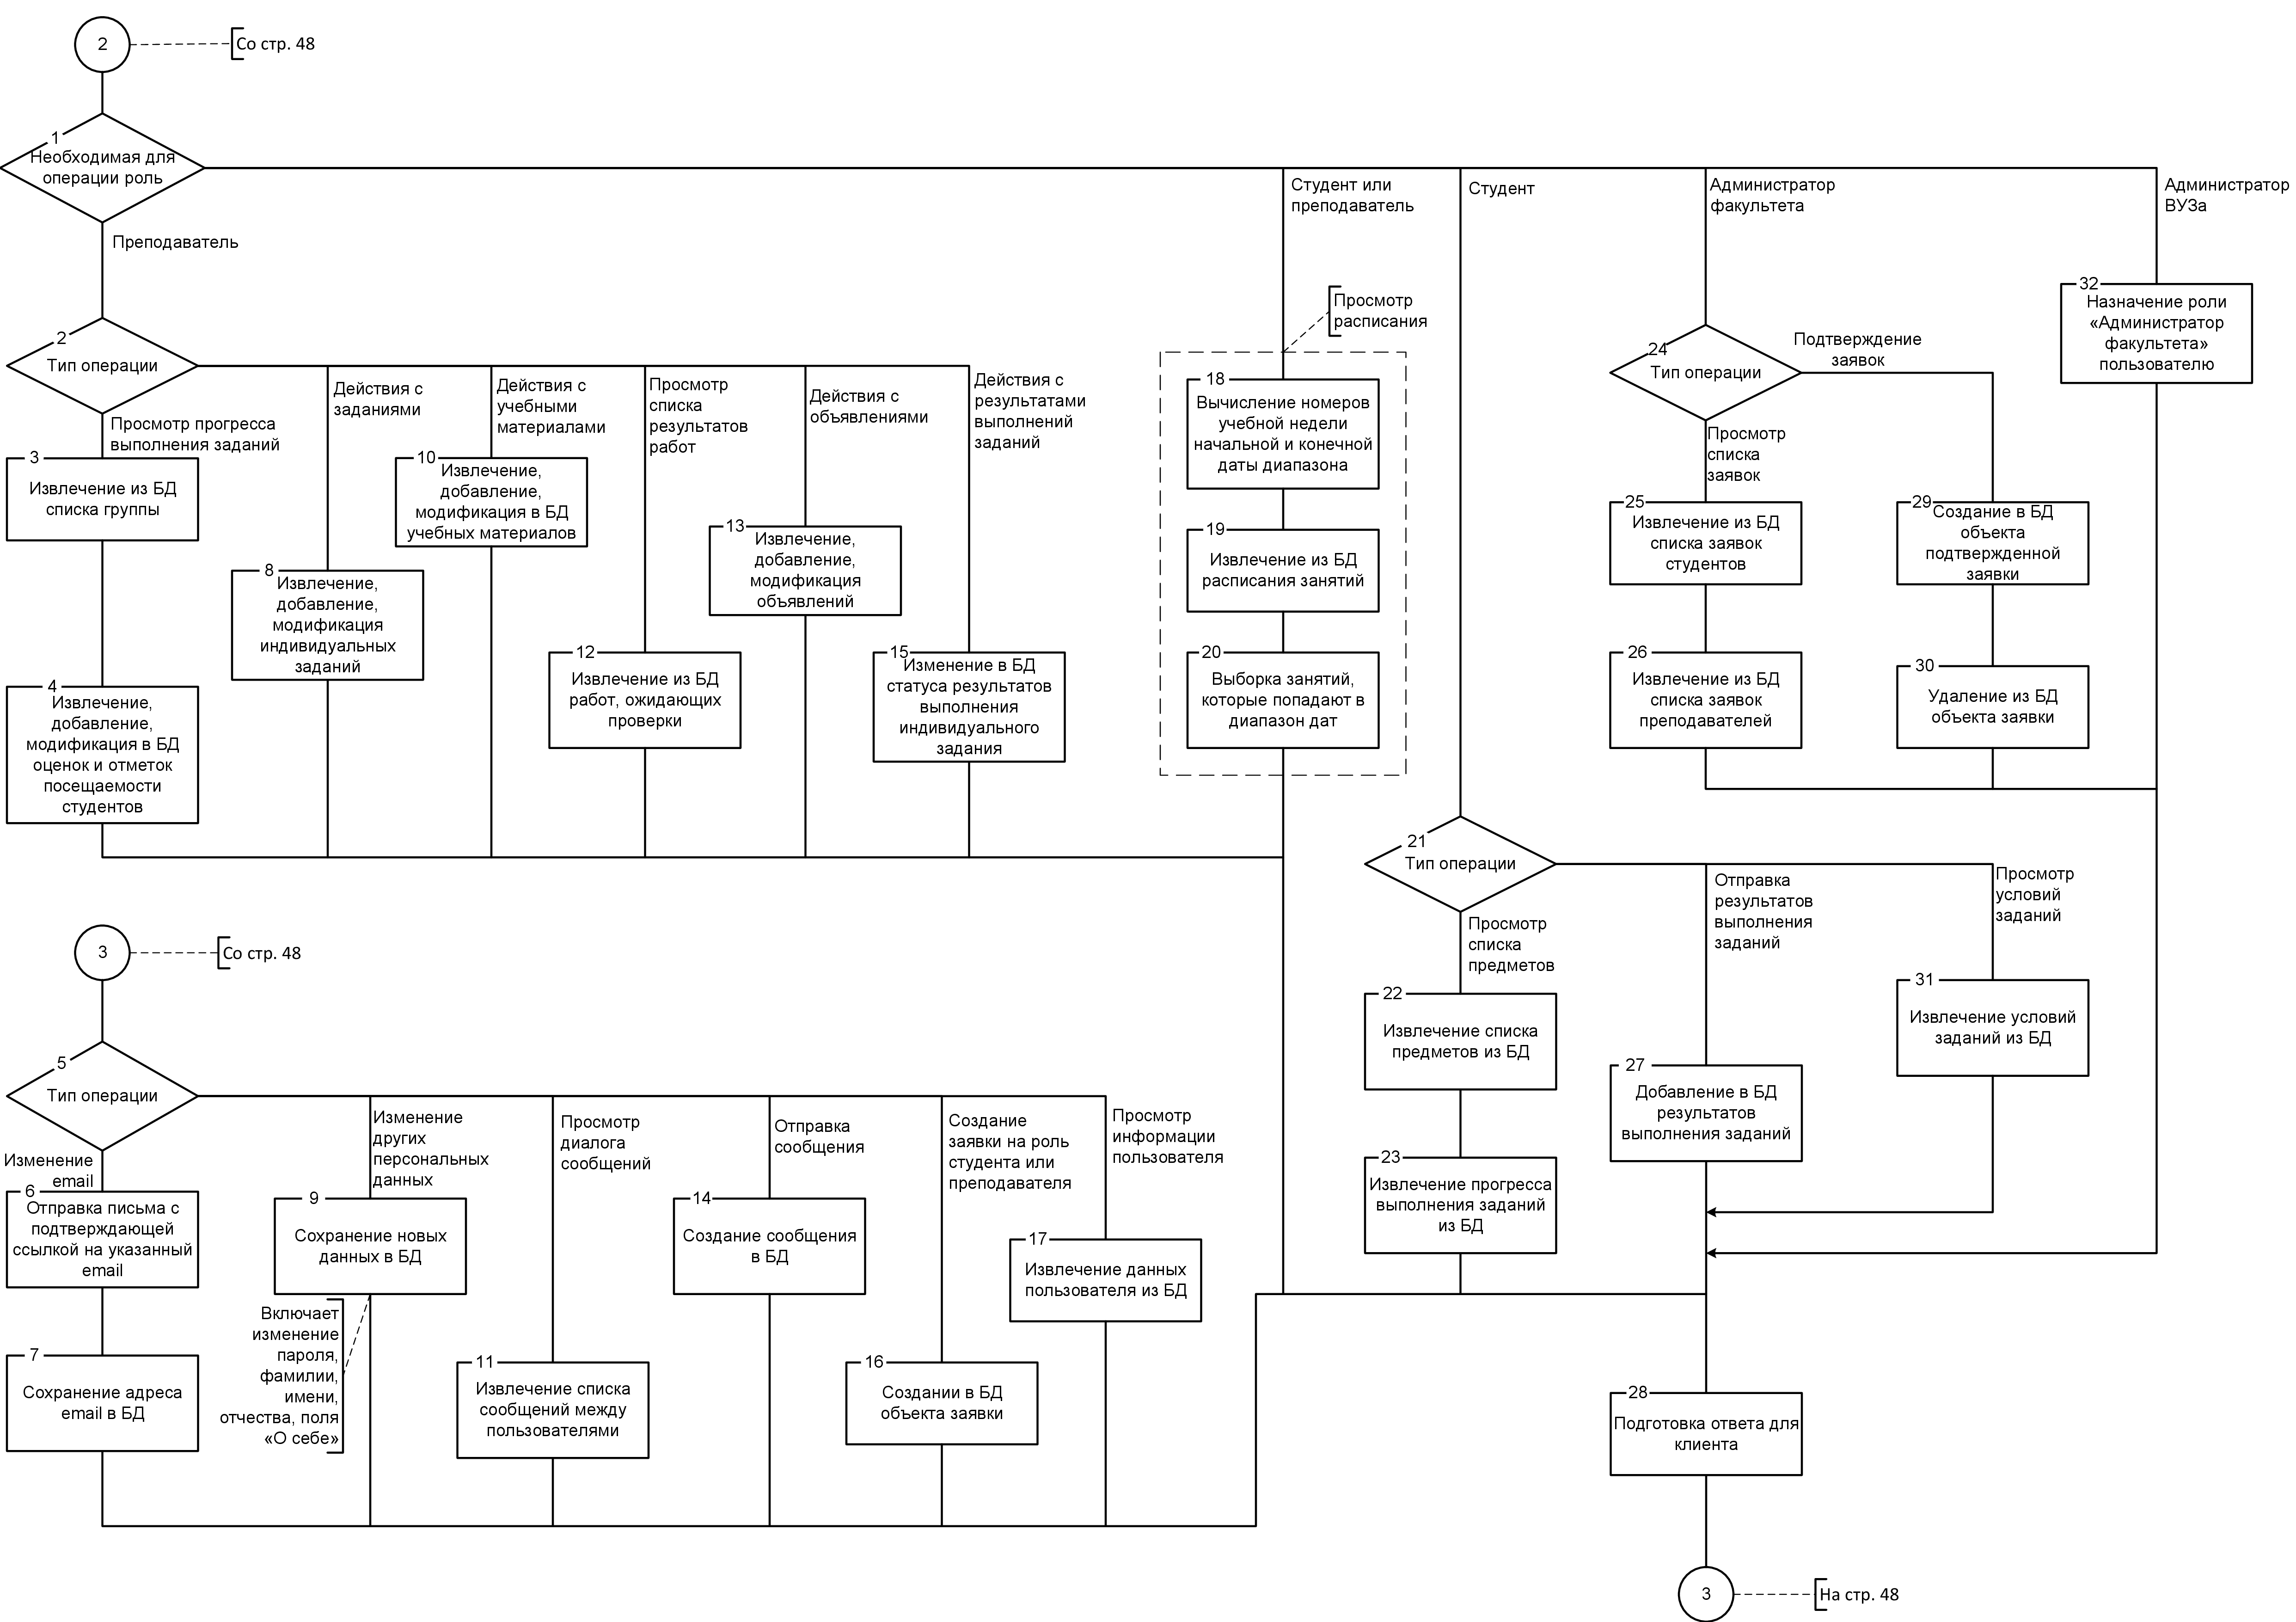
\includegraphics[scale=0.275]{server_algorithm_2.png}
	\caption{Схема программы серверной части программного средства (окончание)}
\end{sidewaysfigure}

Поскольку в ПС проектируется реализация сложных независимых систем ролей и пользовательских функций, которые находят своё отражение в серверной части приложения, то встаёт вопрос об их сопряжении. А поскольку данное сопряжение вследствие особенностей предметной области является достаточно нетривиальным: часть функций уникальна для некоторых функций, часть разделяется ими всеми. Поэтому целесообразным является разбиение их на следующие группы:

\begin{enumerate}
	\item функции, доступные без аутентификации;
	\item функции, доступные для всех аутентифицированных пользователей;
	\item функции студентов;
	\item функции преподавателей;
	\item функции студентов и преподавателей;
	\item функции администраторов факультетов;
	\item функции администраторов ВУЗов.
\end{enumerate}

Часть алгоритма, отвечающее за извлечение расписания занятий из БД, реализована на примере БГУИР, в котором занятия происходят по одной из 4 учебных недель, отсчет которых начинается с 1-го сентября.

Серверная проверка аутентификации пользователей будет осуществляться с помощью технологии создания и проверки специального токена.

Большое количество блоков, в которых осуществляется доступ к БД, подтверждает назначение всей серверной части приложения: прослойка между клиентским веб-приложением и базой данных с добавлением проверок аутентификации и авторизации.

Реализовав перечисленные методы API, можно будет достигнуть очень важной цели: внутренняя бизнес-логика, логика доступа к данным и сами данные будут надежно защищены.

\subsubsection{} Выбор протоколов коммуникации
\label{sec:design:server:protocols}

В пункте~\ref{sec:design:server:overview} приведены этапы, в соответствии с которыми рекомендуется производить проектирование программного системы~\cite{application_architecture_guide}. Этап \ref{sec:design:server:overview}з будет рассмотрен позднее вследствие неоднородности и отсутствия схожести в применяющихся технологий между уровнями. Таким образом, следующий актуальный этап -- \ref{sec:design:server:overview}и: выбор конкретных протоколов взаимодействия.

Можно выделить два основных стиля, которые (с необходимыми модификациями в каждом конкретном случае) применяются в информационных системах, содержащих веб-сервисы~\cite{application_architecture_guide}: REST (Representational State Transfer -- протокол передачи состояния представления) и SOAP (Simple Object Access Protocol -- простой протокол доступа к объектам). Технически REST является архитектурным шаблоном проектирования, построенным на основе использования простых глаголов (называемых запросами или методами). На практике данный архитектурный стиль применяется в связке с протоколом прикладного уровня модели OSI HTTP. SOAP же является XML-ориентированным протоколом, причем стандарт не специфицирует применяемые протоколы передачи данных.

Основное отличие между данными протоколами состоит в способе манипулирования состоянием. SOAP предусматривает осуществление переходов между различными состояниями с помощью взаимодействия с единственной конечной точкой ввода информации, через которую предоставляется доступ к функциональности сервиса. Протокол REST предполагает использование ограниченного набора операций, которые могут применяться к ресурсам, адресуемым с помощью уникальных адресов URI. 

Данный протокол в большей степени соответствует распределенной архитектуре клиент-серверных приложений, поскольку серверная часть публично доступна для множества заведомо неизвестных клиентских приложений. REST обладает свойством отсутствия состояния, что означает, что каждый запрос должен содержать в себе достаточный набор данных для его осуществления. Кроме того, данный протокол не запрещает использование различных форматов передачи данных, например, JSON, что оказывается огромным преимуществом перед SOAP вследствие планируемого использования в клиентской части языка \typescript, который нативно поддерживает данный формат.
